\documentclass[12pt, a4paper]{scrartcl}

\usepackage[utf8]{inputenc}
\usepackage[T1]{fontenc}
\usepackage{lmodern}
\usepackage[ngerman]{babel}
\usepackage{amsmath}
\usepackage{nicefrac}
\usepackage{graphicx, wrapfig, float}
\usepackage[onehalfspacing]{setspace}
\usepackage{paralist}  % \begin{compactitem}

\titlehead{Westfälische Hochschule\\Fachbereich Maschinenbau\vspace{2cm}}
\subject{Entwicklung und Inbetriebnahme einer mikrocontroller-gestützten Ansteuerung eines Roboters mit omnidirektionalem Antrieb}
%Development and implementation of a microcontroller-based control-system for a omnidirectional robotic vehicle.
\title{Projektstudie Robotics \& Automation\vspace{3cm}}
\author{
    \begin{tabular}{rl}
        Manuel Fehmer & 200923513 \\
        Thomas Feldmann & 200923381 \\
        Marlene Feldmann & 200825051 \\
        Carsten Hußmann & 200824460
    \end{tabular}
}

\begin{document}
\maketitle
\newpage
\tableofcontents
\newpage
% !TEX root = Projektstudie.tex
% Einleitung

\section{Einleitung}

Der Mecanum-Roboter ist ein omnidirektionales Fahrzeug. Er kann aus jeder Position in jede beliebige Richtung fahren. Grund dafür sind die verwendeten Allseitenräder - Mecanum-Räder. 

Zur Steuerung des Roboters ist es notwendig ein mathematisches Modell zur Beschreibung der einzelnen Bewegungen der Räder aufzustellen. Abhänging von der Drehrichtung und der Geschwindigkeit der Räder bewegt sich der Roboter.

Bisher werden die Schrittmotoren der Räder mit Hilfe von Nanotec-Treiberkarten und dem CANopen Protokoll angesteuert. Das CANopen Protokoll nutzt als Übertragungsmedium den CAN-Bus. Die Kommunikation läuft über eine SPS. Um die Peripherie zu vereinfachen soll diese durch einen Arduino mit einem CAN-Shield ersetzt werden. Der Austausch soll zudem die Programmierung der Bewegung des Mecanum-Roboters erleichtern.

Ziel der Projektstudie ist es den Austausch durch Entwicklung der notwendigen Treiber zu realisieren, die Bewegung des Roboters über den Arduino zu programmieren und den Roboter über einen Joystick zu steuern. Die omnidirektionale Kinematik soll zudem durch einen Simulator am PC verdeutlicht werden. Ergänzend steht ein weitreichender Ausblick mit ausgearbeiteten Ideen zu einer Platine zur Erweiterung um Sensoren zur Umfelderfassung. 

\subsection*{Vorgehensweise}
In Kapitel eins wird der vorhandene Mecanum-Roboter und die Mecanum-Räder beschrieben. Eine Darstellung der vorgenommenen Hardwaremodifikation erfolgt in Kapitel 2. 
Die Mathematische Modellierung zur Beschreibung der Kinematik und die Treiberentwicklung sind Themen der nächsten zwei Kapitel. Kapitel 5 beschreibt die komplette API inklusive aller Befehle, Fehlercodes und Ereignisse. Die manuelle Steuerung und Simulation werden in Kapitel 6 beschrieben.
Kapitel 7 und 8 bilden den Schlussteil. Nach dem Fazit folgt ein umfassender Ausblick auf mögliche zukünftige Projekte.

\newpage
\begin{figure}[H]
\centering
 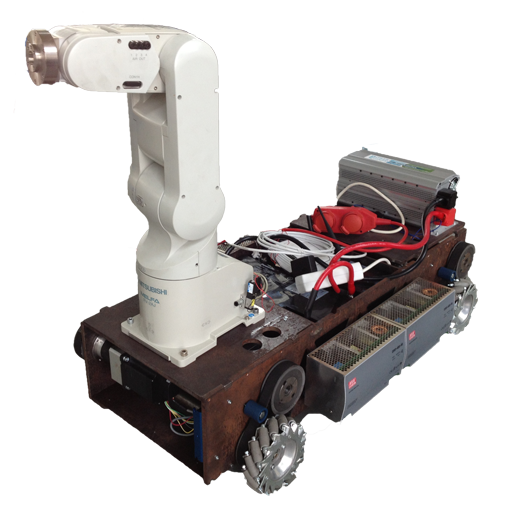
\includegraphics[width=.6\textwidth]{Abbildungen/Roboter} 
\caption[Mecanum-Roboter]{Mecanum-Roboter.}
\label{fig:Roboter}
\end{figure}

\section {Mecanum-Roboter}
\label{sec:Mecanum-Roboter}

Der Mecanum-Roboter ist 1000 mm lang. Er ist mit vier Mecanum-Rädern, die im Rechteck angeordnet sind, ausgestattet. Der Radstand beträgt 775 mm und die Spurbreite beträgt 490 mm. Die Räder haben einen Durchmesser von 115 mm und besitzen jeweils 15 Hilfsrollen. Eine detaillierte Beschreibung folgt im Kapitel \ref{sec:Mecanum-Räder}.

Die Anordnung der Mecanum-Räder und deren Technologie ermöglichen dem Mecanum-Roboter eine omnidirektionale Bewegung. Er kann sich ohne mechanische Lenkung aus jeder Position in jede Richtung fortbewegen.

\subsection*{Mecanum-Räder}
\label{sec:Mecanum-Räder}
Das Mecanum Rad wurde 1973 von der schwedischen Firma Mecanum AB entwickelt und bedient unterschiedliche Anwendungen. Heutige Anwendungsbeispiele sind unter anderem Förderfahrzeuge, fahrerlose Transportfahrzeuge oder Mobilitätshilfe. Auch in der Robotik finden die Allseitenräder immer häufiger Verwendung.
\begin{figure}[H]
\centering
 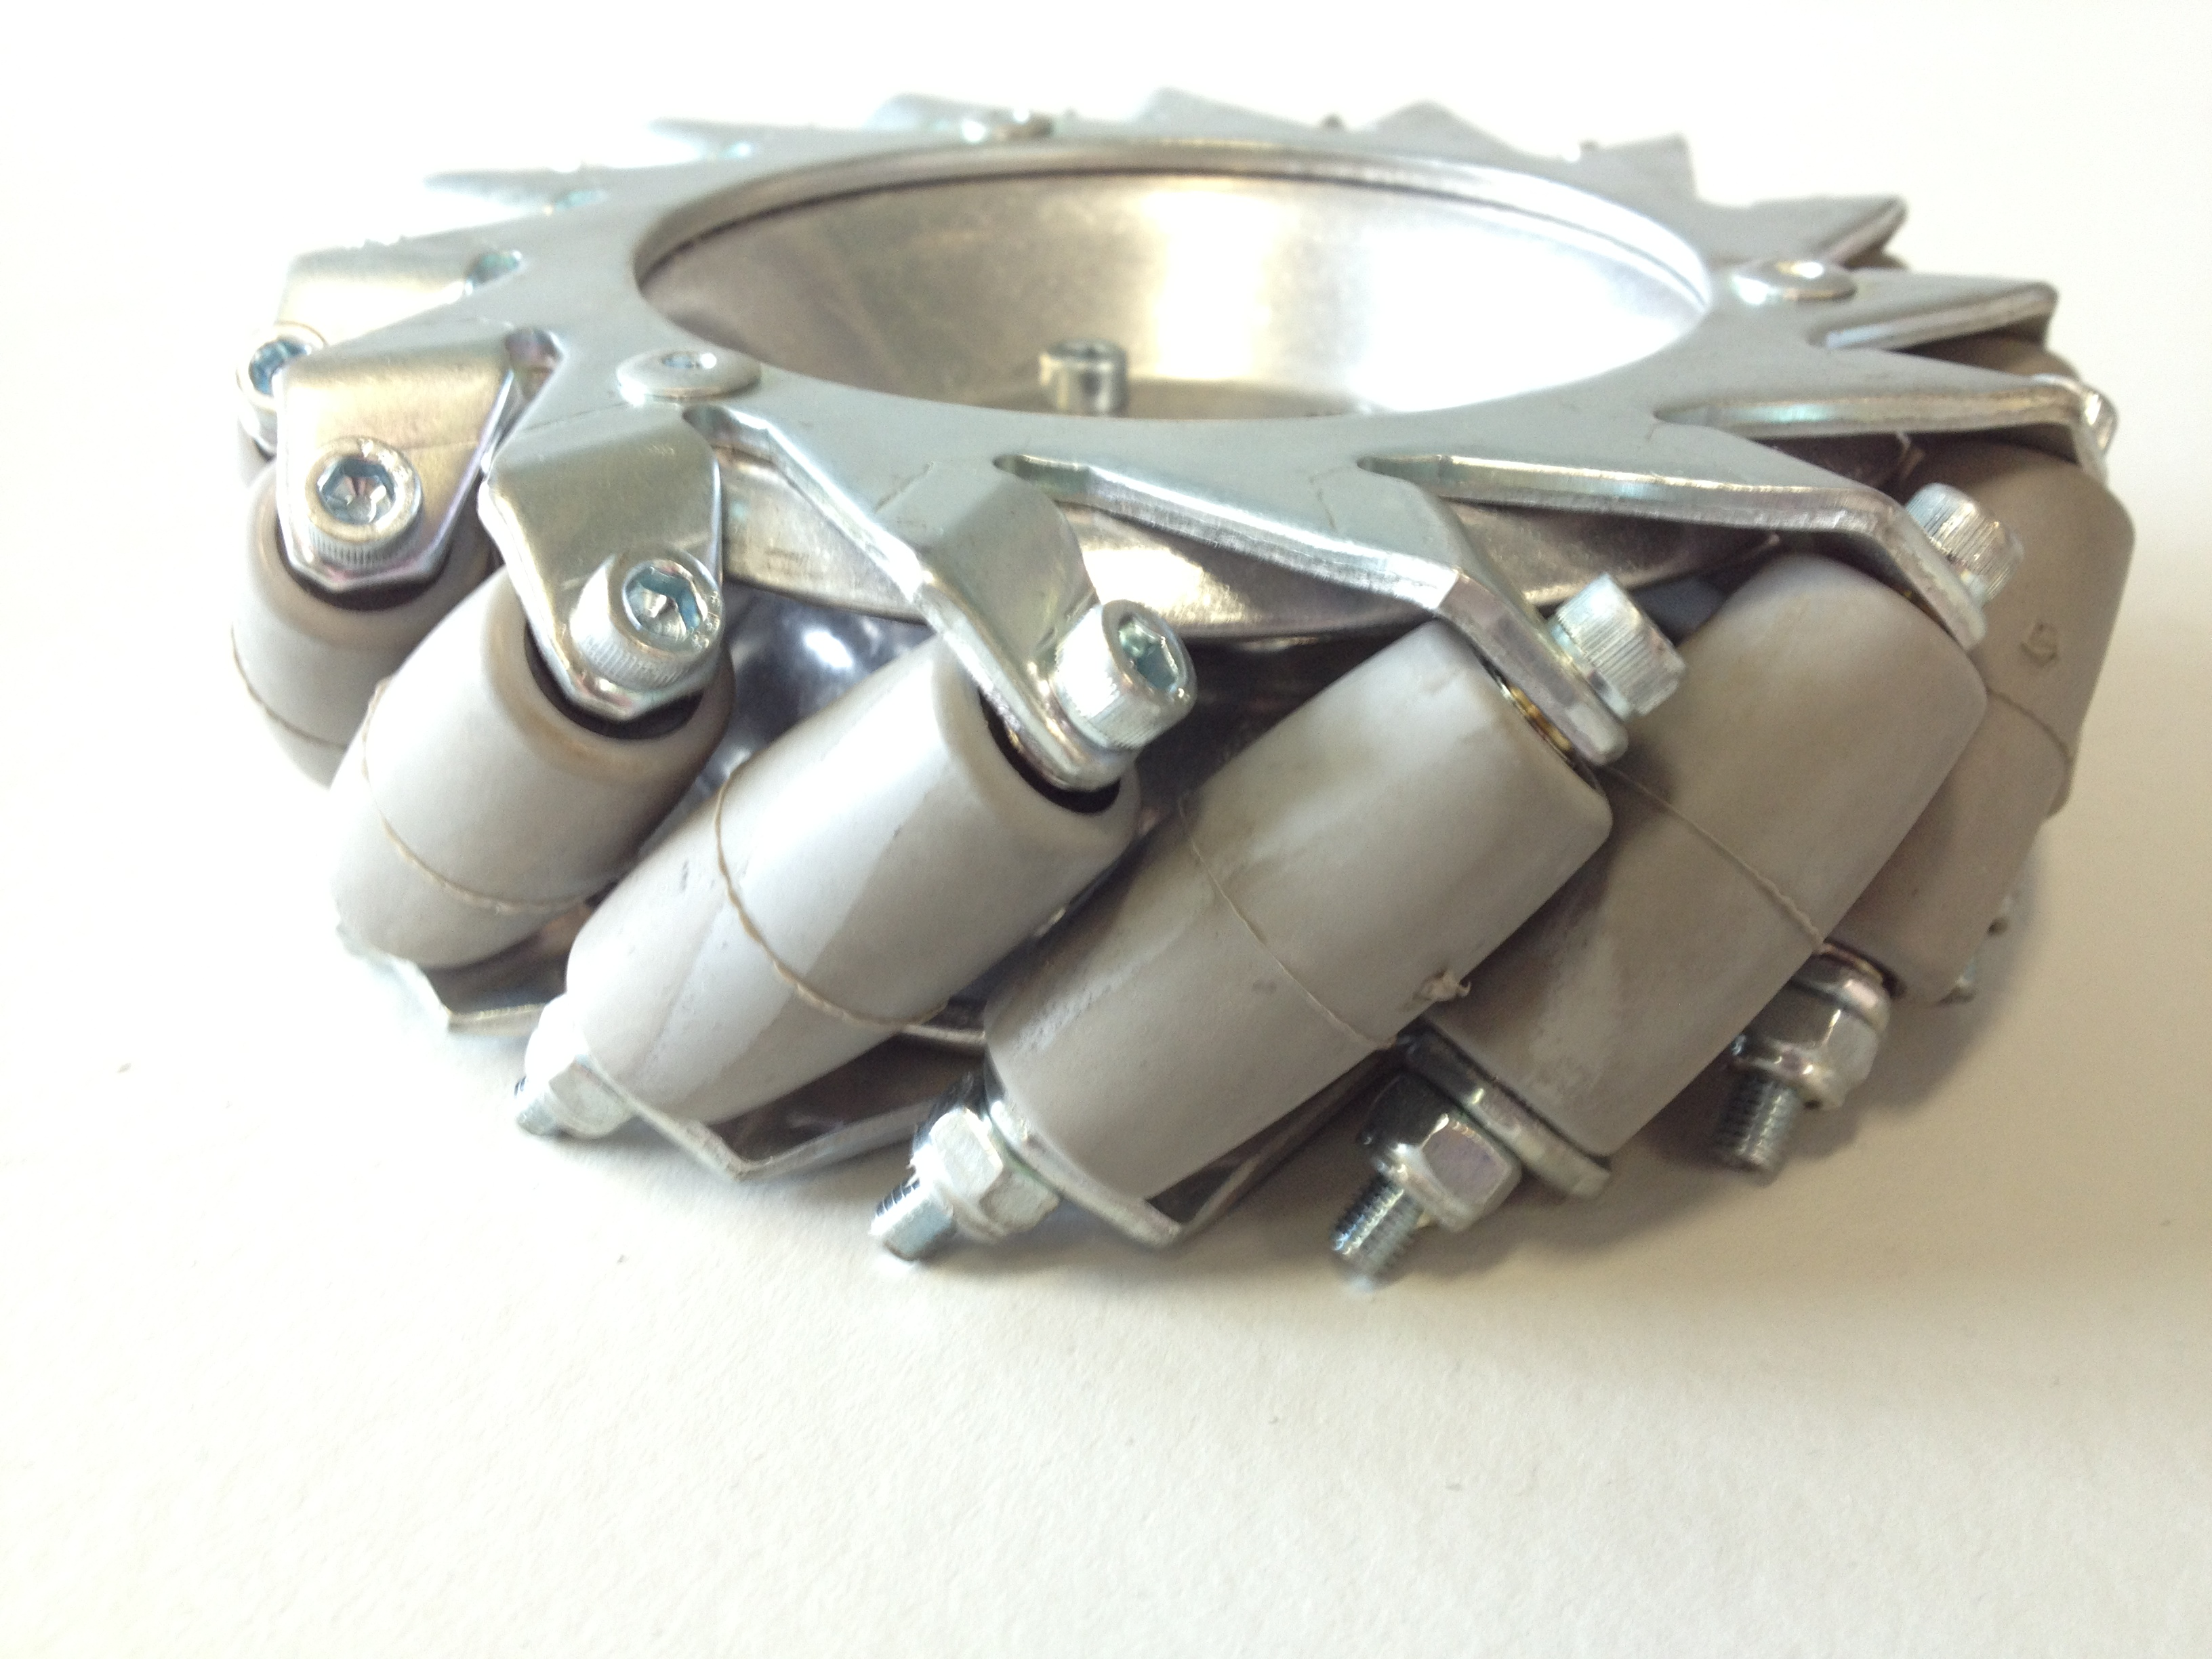
\includegraphics[width=.6\textwidth]{Abbildungen/Mecanumrad} 
\caption[Mecanum-Rad]{Mecanum-Rad.}
\label{fig:Mecanum-Rad}
\end{figure}
Abbilung \ref{fig:Mecanum-Rad} zeigt ein Mecanum-Rad des Mecanum-Roboters. Auf dem Umfang des Rades sind 15 tonnenförmige beschichtete Rollen im Winkel von 45 Grad zur Radachse angebracht. Diese Rollen haben keinen eigenen Antrieb und sind frei drehbar gelagert. Ausschließlich die Rollen haben Kontakt zum Boden.
Jedes Mecanum-Rad wird von einem Schrittmotor angetrieben. Somit sind Drehsinn und Drehzahl für jedes Rad einzeln ansteuerbar. Dieses ist entscheidend für die omnidirektionale Bewegung.
Durch eine individuelle Drehrichtungsauswahl entstehen durch die Hilfsrollen am Untergrund Kraftvektoren in unterschiedliche Richtungen. Die Summe der Vektoren aller Räder bildet die Gesamtbewegungsrichtung oder auch ein Gesamtdrehmoment.






















% !TEX root = Projektstudie.tex
% Mathematik


\section{Mathematische Modellierung}
\label{sec:Mathematische Modellierung}
%\Delta
\begin{figure}
    \centering
    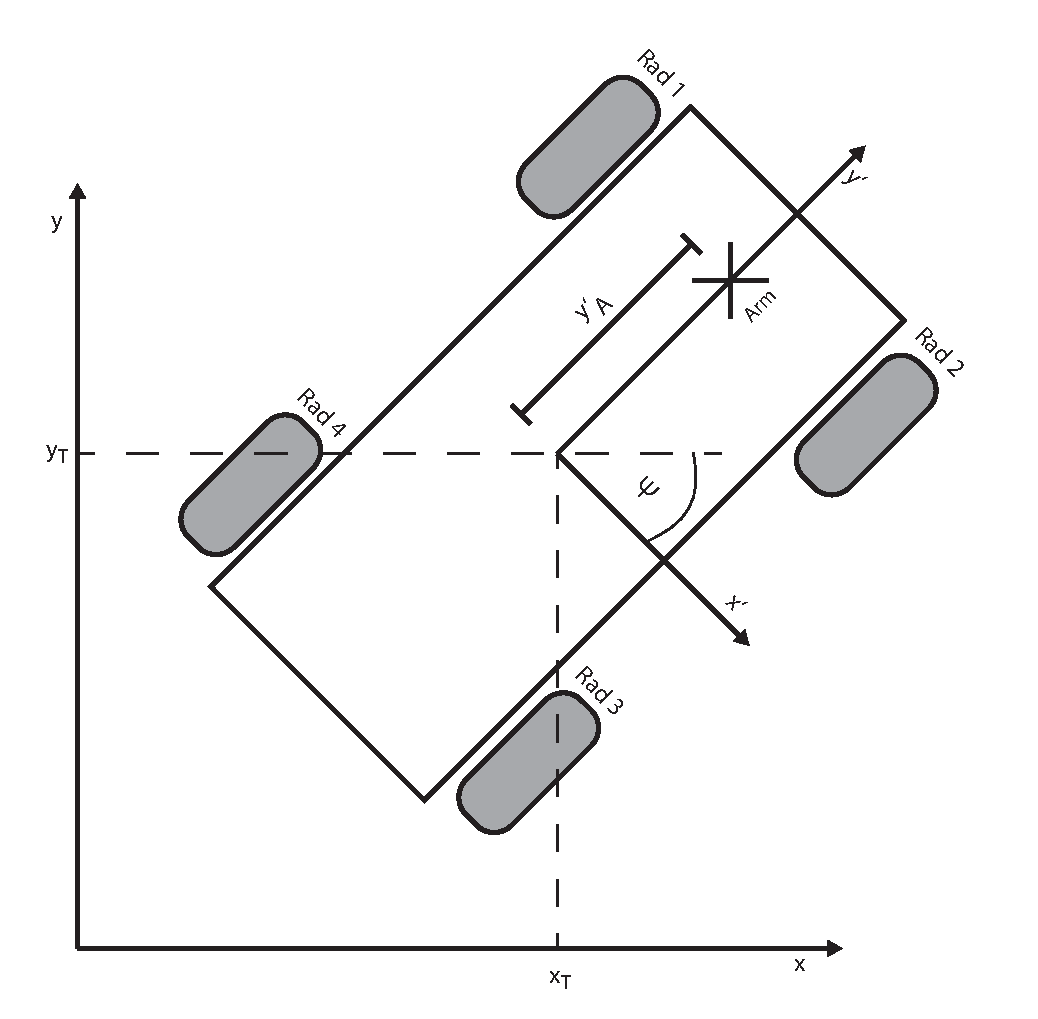
\includegraphics[width=.8\textwidth]{Abbildungen/Koordinaten}
    \caption{Einführung der verwendeten Koordinatensysteme, der Position des Arms sowie der Radnummerierung.}
\end{figure}
Dieses Kapitel beschreibt die Mathematik hinter der Kinematik und Dynamik des Mecanum-Roboters.
Jede Bewegung setzt sich aus einer translatorischen und einer rotatorischen Teilbewegung zusammen. Abbildung\ref{fig:Drehrichtung} zeigt die Raddrehrichtungen und die daraus resultierenden Roboterbewegungen.

\begin{figure}[H]
    \centering
    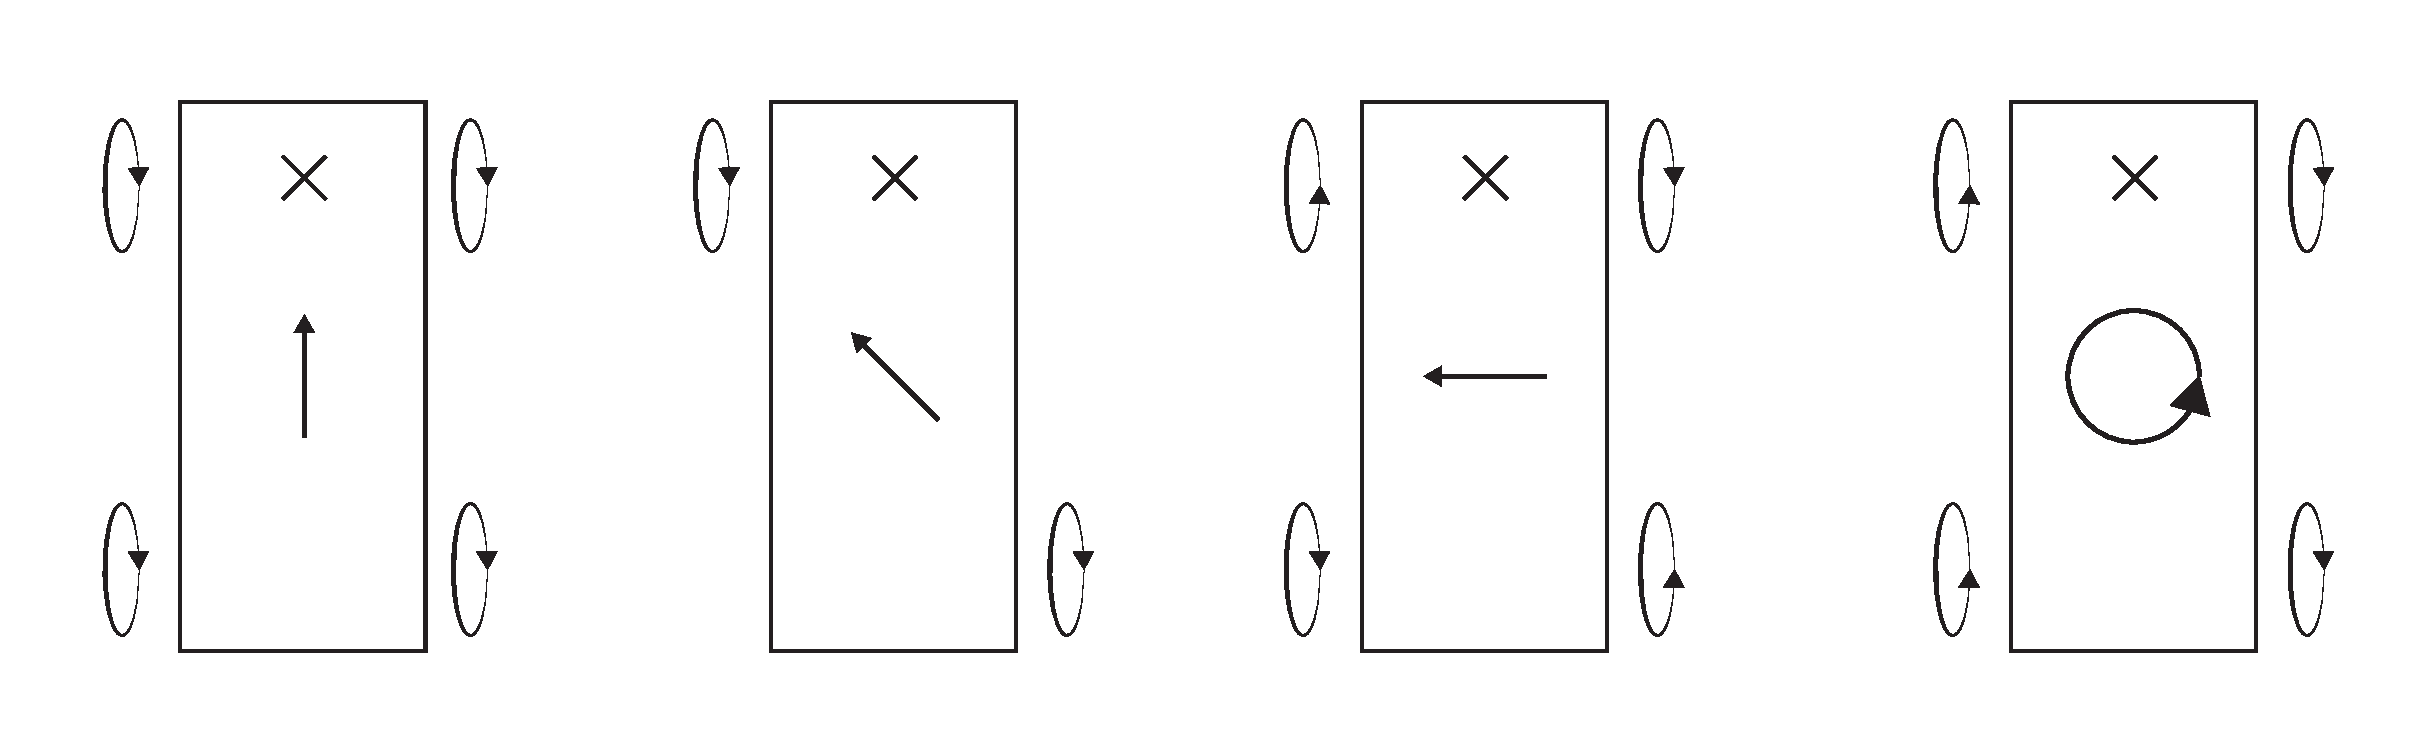
\includegraphics[width=.8\textwidth]{Abbildungen/Drehrichtung}
    \caption{Darstellung der Raddrehrichtungen und der resultierenden Bewegungen.}
    \label{fig:Drehrichtung}
\end{figure}

\subsection{Translation}
\label{sec:Translation}
Um eine translatorische Bewegung auszuführen, werden die Räder paarweise (1+3, 2+4) mit gleicher Drehrichtung und Drehgeschwindigkeit angetrieben.
Die resultierende Gesamtkraft bestimmt die Richtung der Fahrt.
Die folgenden Rechnungen behandeln die Ermittlung der einzelnen Soll-Radgeschwindigkeiten aus einem vorgegebenen Geschwindigkeitsvektor.

\begin{figure}[H]
    \centering
    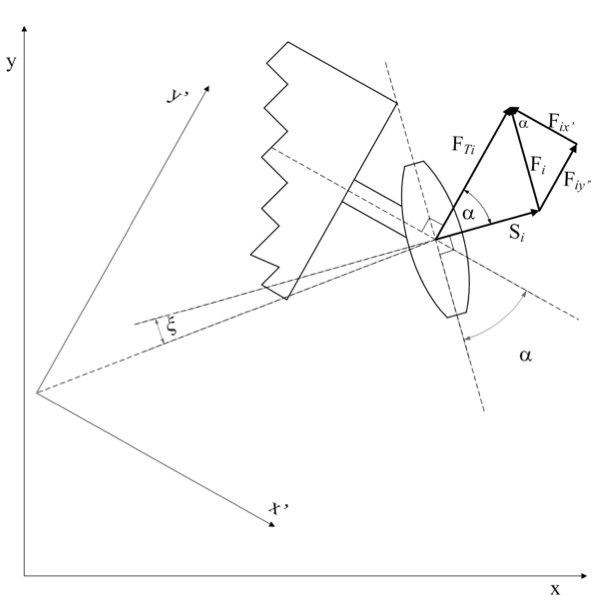
\includegraphics[width=.6\textwidth]{Abbildungen/Kraefte-am-Rad}
    \caption{Kräftegleichgewicht an einem Mecanum-Rad.}
\end{figure}

Die Leistung einer vektoriellen Kraft berechnet sich nach : 
$$ P_F = F_T \cdot v_F $$

Wirken Kraft und Geschwindigkeit entlang einer Koordinatenachse, haben beide Vektoren die gleiche Komponente ungleich null und ihr Skalarprodukt kann vereinfacht als Produkt der skalaren Größen betrachtet werden.

Die Kraftvektor in $x$- und $y$-Richtung setzt sich zusammen als die Summe der einzelnen $x$- und $y$-Vektoren der vier Räder:
\begin{align*}
    \sum_{i=1}^4 F_{ix} &= \sum_{i=1}^4 F_i \cos \alpha \\
    &= \sum_{i=1}^4 (-1)^i SIG \cdot K_i F_{Ti} \sin \alpha \cos \alpha \\
    &= \sum_{i=1}^4 (-1)^i SIG \cdot \frac{1}{2} K_i F_{Ti}
\end{align*}
\begin{align*}
    \sum_{i=1}^4 F_{iy} &= \sum_{i=1}^4 F_i \sin \alpha \\
    &= \sum_{i=1}^4 SIG \cdot K_i F_{Ti} \sin^2 \alpha \\
    &= \sum_{i=1}^4 SIG \cdot \frac{1}{2} K_i F_{Ti}
\end{align*}

SIG sei die Vorzeichenkonventionen für die Drehrichtung der Räder.
Diese wird in der Steuerung direkt implementiert und wird daher bei den folgenden Rechnungen nicht weiter betrachtet.

Der Winkel $ \alpha $ beschreibt den Winkel, in dem die Rollen auf dem Mecanum-Rad angebracht sind.
In den meisten Fällen gilt $\alpha = 45^\circ$.

Für eine translatorische Bewegung müssen die Radpaare mit gleicher Geschwindigkeit drehen.
Entsprechend müssen ihre Kraftvektoren $F_{T1, 3} / F_{T2, 4}$ gleich groß sein.
Durch Auflösen der Summenzeichen erhält man ein Gleichungssystem:
\begin{align*}
    F_x &= - K_i F_{T1, 3} + K_i F_{T2, 4} \\
    F_y &= K_i F_{T1, 3}   + K_i F_{T2, 4}
\end{align*}

Nach dem Umstellen erhält man $F_{T1, 3}$ und $F_{T2, 4}$ und kann somit auch direkt die Geschwindigkeiten berechnen:
\begin{align*}
    F_{T1, 3} &= \frac{F_y + F_x}{K_i} &\Rightarrow v_{T1, 3} &= \frac{v_y + v_x}{K_i} \\
    F_{T2, 4} &= \frac{F_y - F_x}{K_i} &\Rightarrow v_{T2, 4} &= \frac{v_y - v_x}{K_i} \\
\end{align*}

Der Faktor $K_i$ setzt sich aus unterschiedlichen Einzelfaktoren zusammen, welche die durch das Motormoment erzeugten treibenden Kräfte beeinflussen. $K_i$ wird für den Boden der Werkstatt empirisch ermittelt. Die Beschreibung der durchgeführten Versuchsreihe folgt in Kapitel~\ref{sec:versuche-k-faktor}.


\subsection{Rotation}
\label{sec:Rotation}
Die Rotation des Mecanum-Roboters um sein Zentrum müssen alle Räder mit gleicher Geschwindigkeit drehen, lediglich die Richtung unterscheidet sich.
Für eine Drehung im Uhrzeigersinn drehen beispielsweise Rad 1 und 2 rückwärts, Rad 3 und 4 vorwärts. Allgemein gilt:
\begin{align*}
    v_{ref} &= K_i \cdot r \cdot \omega \\
    v_1 = v_4 &= - v_{ref} \\
    v_2 = v_3 &= + v_{ref}
\end{align*}

\subsection{Betrachtung $K_i$}
\label{sec:k-faktor}

Der Faktor $K_i$ hat einen großen Einfluss auf die Bewegung des Mecanum-Roboters. Er setzt sich aus unterschiedlichen Einzelfaktoren zusammen, welche die durch das Motormoment erzeugten treibenden Kräfte beeinflussen. Zu den Einflussfaktoren zählen unter anderem die verschiedenen Reibungsfaktoren und die Flächenträgheitsmomente. 

Da eine Bestimmung der einzelnen Faktoren sehr aufwendig ist und die Varianzen der Fehleranteile  bei der Multiplikation zu $K_i$ ebenfalls multipliziert werden müssen, ist eine direkte Bestimmung von $K_i$ zu empfehlen. Die Bestimmung von  $K_i$ muss zudem explizit für den Untergrund auf dem der Roboter fahren soll erfolgen. Der Einfluss weiterer Einflussfaktoren (Feuchtigkeit, Staub, etc.) sollte durch definierte Randbedingungen möglichst gering gehalten werden. 
Da die Reibung auch von der Auflagefläche der Rollen abhängig ist und diese je nach Fahrtrichtung (siehe Abbilung \ref{fig:himmel}) variiert, wird ein zusätzlicher Einfluss der Fahrtrichtung auf  $K_i$ vermutet. 

\begin{figure}[H]
    \centering
    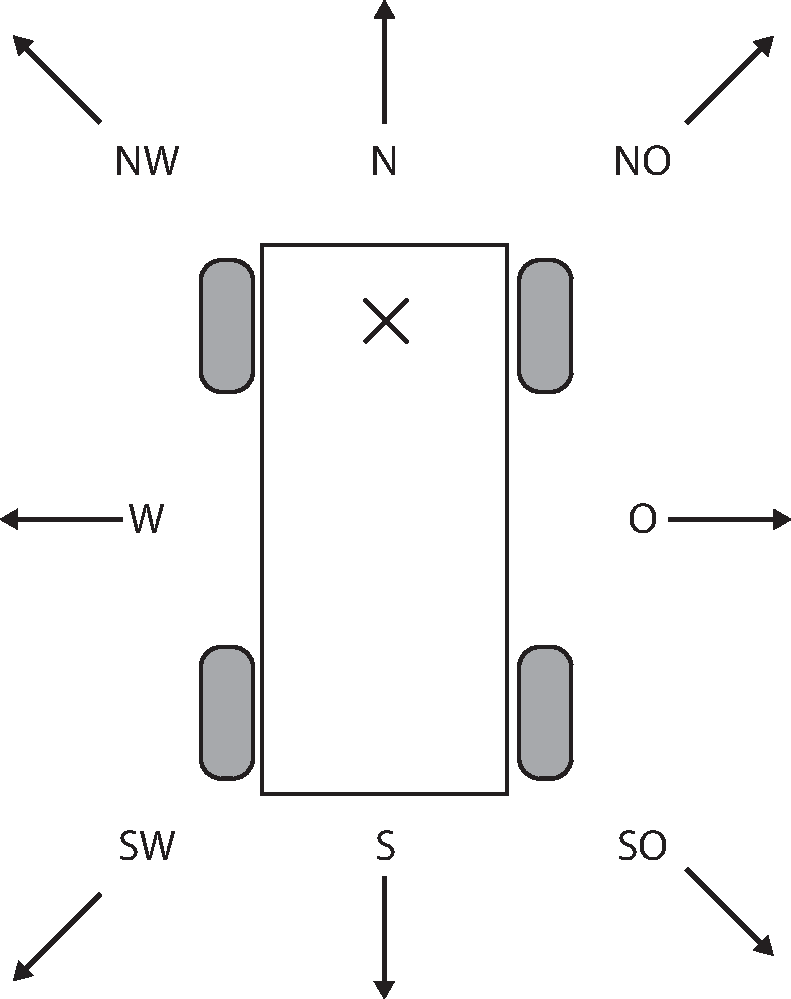
\includegraphics[width=.4\textwidth]{Abbildungen/Himmelsrichtungen}
    \caption{Orientierung des Roboters}
    \label{fig:himmel}
  \end {figure}

Unebenheiten, welche aufgrund der Funktionsweise der Mecanum-Räder ebenfalls einen großen Einfluss haben, können aus Praktikabilitätsgründen bei optionalen Versuchsreihen nicht berücksichtigt werden. 

Aufgrund der vielen Variablen und des erhöhten Zeitaufwandes wird auf eine genaue Bestimmung des Faktors $K_i$ an dieser Stelle verzichtet. 













% !TEX root = Projektstudie.tex

% !TEX root = Projektstudie.tex
% Treiber


\section{Treiberentwicklung}
\label{sec:Treiber}

Die Schrittmotortreiber der Firma Nanotec arbeiten mit dem CANopen Protokoll. Zur Ansteuerung der Motoren sind verschiede Befehle notwendig, die im Folgenden kurz beschrieben werden. Damit der richtige Motor angesteuert wird, müssen diese Befehle an die richtige COB-ID gesendet werden. Die COB-ID setzt sich aus der 0x600 und der jeweiligen Node-ID der Schrittmotorkarte zusammen. Die Node-ID kann an der Unterseite der Schrittmotortreiberkarten über zwei Drehschalter eingestellt werden.

Beispiel:
Ein Motor mit der Node-ID 3 wird über die COB-ID 0x603 angesteuert.


\subsection*{Befehlsaufrufe}

Vor dem Start der Motoren muss das Leistungsteil eingeschaltet und der richtige Operationsmodus gewählt werden. Tabelle~\ref{tab:velocitymode} zeigt, wie die Treiberkarte in den \emph{Velocity Mode} versetzt wird. Anschließend werden (Tabelle~\ref{tab:velmodesettings}) die Einstellungen im Velocity Mode vorgenommen.

\begin{table}[H]
    \begin{tabularx}{\textwidth}{@{}Xl@{}} \toprule


    Befehl & Code \\
    \midrule

    Switch on Disabled (Grundzustand)  &
    \lstinline{0x2B 0x40 0x60 0x00 0x00 0x00 0x00 0x00} \\

    Ready to Switch on  &
    \lstinline{0x2B 0x40 0x60 0x00 0x06 0x00 0x00 0x00} \\

   Switch on  &
    \lstinline{0x2B 0x40 0x60 0x00 0x07 0x00 0x00 0x00} \\

    Operation Enabled  &
    \lstinline{0x2B 0x40 0x60 0x00 0x0F 0x00 0x00 0x00} \\

    \bottomrule
    \end{tabularx}
    \caption{Leistungsteil einschalten}
\end{table}


\begin{table}[H]
    \begin{tabularx}{\textwidth}{@{}Xl@{}} \toprule


    Befehl & Code \\
    \midrule

    Velocity Mode auswählen &
    \lstinline{0x2F 0x60 0x60 0x00 0x02 0x00 0x00 0x00} \\

    \bottomrule
    \end{tabularx}
    \caption{Operationsmodus auswählen}
    \label{tab:velocitymode}
\end{table}


\begin{table}[H]
    \begin{tabularx}{\textwidth}{@{}Xl@{}} \toprule

    Befehl & Code und Beispiel \\
    \midrule

    Minimale Geschwindigkeit einstellen &  \ttfamily{0x23 0x46 0x60 0x01 \textcolor{blue}{0x00 0x00} 0x00 0x00} \\
    & Hier: \ttfamily{\textcolor{blue}{0x0000}} = 0 Schritte/s \\

    Maximale Geschwindigkeit einstellen &  \ttfamily{0x23 0x46 0x60 0x02 \textcolor{blue}{0xA8 0x61} 0x00 0x00} \\
    & Hier: \ttfamily{\textcolor{blue}{0x61A8}} = 25000 Schritte/s \\

    \textbf{Beschleunigungsrampe\footnotemark\addtocounter{footnote}{-1}:} \\


    Geschwindigkeitsänderung einstellen &  \ttfamily{0x23 0x48 0x60 0x01 \textcolor{blue}{0x20 0x4E} 0x00 0x00} \\
    & Hier: \ttfamily{0x4E20} = 20000 Schritte/s \\


    Zeitänderung einstellen &  \ttfamily{0x2B 0x48 0x60 0x02 \textcolor{blue}{0x01 0x00} 0x00 0x00} \\
    & Hier: \ttfamily{0x0001} = 1 s \\

    \textbf{Bremsrampe\footnotemark\addtocounter{footnote}{-1}:} \\

     Geschwindigkeitsänderung eintellen &  \ttfamily{0x23 0x49 0x60 0x01 \textcolor{blue}{0x20 0x4E} 0x00 0x00} \\
    & Hier: \ttfamily{0x4E20} = 20000 Schritte/s \\

    Zeitänderung einstellen  &  \ttfamily{0x2B 0x49 0x60 0x02 \textcolor{blue}{0x01 0x00} 0x00 0x00} \\
    & Hier: \ttfamily{0x0001} = 1 s \\

    \textbf{Bremsrampe\footnotemark:} \\
    (Für Quick-Stop) \\

     Geschwindigkeitsänderung eintellen &  \ttfamily{0x23 0x4A 0x60 0x01 \textcolor{blue}{0xA0 0x86} 0x00 0x00} \\
    & Hier: \ttfamily{0x86A0} = 34464 Schritte/s \\

    Zeitänderung einstellen  &  \ttfamily{0x2B 0x4A 0x60 0x02 \textcolor{blue}{0x01 0x00} 0x00 0x00} \\
    & Hier: \ttfamily{0x0001} = 1 s \\

    \bottomrule
    \end{tabularx}
    \caption{Einstellungen im Velocity Mode}
    \label{tab:velmodesettings}
\end{table}
\footnotetext{angegeben in Geschwindigkeitsänderung pro Zeitänderung }

Ist die Initialisierung abgeschlossen, kann mit folgendem Befehl die Geschwindigkeit des Schrittmotors in Schritte pro Sekunde eingestellt werden.

\begin{table}[H]
    \begin{tabularx}{\textwidth}{@{}Xl@{}} \toprule

    Befehl & Code und Beispiel \\
    \midrule

    Geschwindigkeit einstellen &  \ttfamily{0x2B 0x42 0x60 0x00 \textcolor{blue}{0x10 0x27} 0x00 0x00} \\
    & Hier: \ttfamily{0x2710} = 10000 Schritte/s \\

    \bottomrule
    \end{tabularx}
    \caption{Geschwindigkeit einstellen}
\end{table}




% !TEX root = Projektstudie.tex
% API

\section{API}
Die Kommunikation mit dem Roboter findet über die UART-Schnittstelle bei einer Baudrate von 115200 Mbaud statt.
Auf dem Arduino sorgt die Library \emph{SerialCommand}\footnote{https://github.com/kroimon/Arduino-SerialCommand} für die Interpretation der Ergebnisse.

\subsection{Befehle}
Folgende Befehle sind verfügbar:
\begin{description}
\item \lstinline{@start} \\
Initialisiert und startet die Schrittmotor-Treiberkarten gemäß Kapitel~\ref{sec:Treiber}.
Der Roboter ist daraufhin fahrbereit.

\item \lstinline{@stop} \\
Führt einen Not-Stopp durch. Dabei wird der in Kapitel~\ref{sec:Treiber} beschriebene Quickstop ausgeführt.
Anschließend befinden sich die Schrittmotor-Treiberkarten im Ruhezustand und müssen erst wieder mit dem Befehl \lstinline{@start} gestartet werden.

\item \lstinline{@v v1 v2 v3 v4} \\
Über diesen Befehl werden die Soll-Radgeschwindigkeiten vorgegeben.

Anstelle von \lstinline{v1, v2, v3} und \lstinline{v4} sind durch Leerzeichen getrennte, ASCII-codierte Integer im Bereich von $-25000$ bis $25000$ (Schritte pro Sekunde) anzugeben.
\end{description}


\subsection{Fehlercodes}
Tritt bei der Kommunikation mit der API ein Fehler auf, führt der Roboter sofort einen Not-Stopp aus und antwortet mit einem Fehlercode sowie einer Fehlerbeschreibung.
Damit ist auch bei einer Störung der Kommunikation gewährleistet, dass der Roboter nicht außer Kontrolle gerät.
Mögliche Fehlercodes sind beispielsweise:

\lstinline{!E01: Not enough arguments supplied.}\\
\lstinline{!E02: Unknown command: [command]}\\


\subsection{Ereignisse}
Um externer Software Rückschlüsse auf den Zustand des Roboters zu ermöglichen, sendet dieser bei erfolgreichen Initialisierungen oder Befehlen Ereignisprotokolle.

Fest definierte, für die steuernde Software relevante Aktivitäten werden mit vorangestelltem Index gesendet:\\
\lstinline{@A01: All motors are ready.}\\
\lstinline{@A02: New motor speed set.}\\
\lstinline{@A03: QuickStop successful.}

Sonstige Logging-Nachrichten werden mit einer Raute versehen.
Dazu zählen aktuelle Soll-/Ist-Werte und Informationen über die Firmware, wie beispielsweise\\
\lstinline{# Left: 120, Right: 230}\\
\lstinline{# Firmware Version 1.0, compiled on Tue Jun  4 18:15:59 2013}

% !TEX root = Projektstudie.tex
% Simulator

\section{Simulator}

% !TEX root = Projektstudie.tex
% Fazit

\section{Fazit}
\label{sec:Fazit}

Während zahlreicher Versuchsfahrten stellt sich heraus, dass eine  genaue Positionierung nur mit Kenntnis der Radgeschwindigkeiten keine möglich ist. Kleinste Unebenheiten oder Verschmutzungen resultieren in durchrutschenden oder abhebenden Rädern und somit in starken Fahrbahnabweichungen. Für den produktiven Betrieb sind daher externe Positionsreferenzen zwingend notwendig. Weitere Ausführungen dazu folgen im Ausblick Kapitel~\ref{sec:Ausblick}.

Neben dem Fahrbahnuntergrund erschweren mechanische Probleme ein reibungsloses Fahren des Mecanum-Roboters: 

\begin{itemize}
    \item{Die Motoren sind zu schwach dimensioniert und verlieren bei abrupten Manövern Schritte.}
    \item{Das treibende Rad des Riementriebs löst sich nach längerem Gebrauch von der Welle und muss mit gezielten Hammerschlägen wieder an seine Position gebracht werden. Dies hat zur Folge, dass die Mecanum-Räder zu nah am Riementrieb liegen und sich regelmäßig mit den überstehenden Schrauben im Riemen verhaken.}
\end{itemize}

Ein Beheben dieser Probleme setzt eine Neukonstruktion der betrachteten Komponenten voraus. Weitere notwendige Änderungen werden neben Optimierungsansätzen und möglichen folgenden Projekten im Ausblick Kapitel~\ref{sec:Ausblick} beschrieben.

% !TEX root = Projektstudie.tex
% Ausblick

\section{Ausblick}
\label{sec:Ausblick}
Im Ausblick werden zu den Punkten Schutzbeschaltung, Neukonstruktion, Arduino-Shield und Drahtlose Navigation auf dem Betriebsgelände Anregungen gegeben um das Projekt zu optimieren.

\subsection{Schutzbeschaltung}
\label{sec:Schutzbeschaltung}
%NOT-AUS
Um einen sicheren Betrieb des Roboters sicher zu stellen, muss ein NOT-AUS-Schalter nachgerüstet werden. Dieser muss in der Lage sein jede Bewegung des Roboters zu beenden.
\begin{itemize}
\item{Im Netzbetrieb an einer Verlängerungsleitung muss der NOT-AUS-Schalter den Roboter von der Netzspannung trennen.}
\item{Im Akkubetrieb muss der NOT-AUS-Schalter beide Pole vom Akku abschalten.}
\end{itemize}
In beiden Fällen muss der NOT-AUS-Schalter die vorhandenen Ströme sicher abschalten können. Des Weiteren sollten Sicherungsautomaten und Schutz gegen Berühren von spannungsführenden Teilen und Quetschgefahrstellen nachgerüstet werden.

\subsection{Neukonstruktion}
\label{sec:Neukonstruktion}
Um die im Fazit Kapitel \ref{sec:Fazit} beschriebenen Probleme zu beheben, empfiehlt sich eine Neukonstruktion des Mecanum-Roboters.
\begin{itemize}
\item{Um permanenten Bodenkontakt mit allen vier Rädern,welcher essentiell für die Funktionsweise der Mecanum-Räder ist, zu gewährleisten sollte eine Einzelradaufhängung oder eine Pendelachse vorgesehen werden.}
\item{Da die Motortreiberkarten mit $48V$ bereits an der oberen Leistungsgrenze betrieben werden, könnte man die mangelnde Motorleistung durch Reduktion der Gesamtmasse ausgleichen. Dies könnte man durch diverse Maßnahmen realisieren:
\begin {itemize}
\item{Konstruktion des Chassis aus einem leichtern Werkstoff wie z.\,B.\ Aluminium.}
\item{Durch einen $48V$-Akku können DC-AC-Konverter und die vier Netzteile eingespart werden.}
\end{itemize}
}
\item{Axiale Sicherung der Riemenscheiben auf den Motorwellen und Kürzung der überstehenden Schraubenenden an den tonnenförmigen Umfangsrollen der Mecanum-Räder.}
\item{Zur besseren Navigation sollte der Schwerpunkt im Mittelpunkt des Roboters liegen und der Radstand gleich der Spurbreite sein.}
\end{itemize}

\subsection{Arduino-Shield}
\label{sec:Arduino-Shield}
% - Arduino-Shield
Da der Speicher des verwendeten Arduino UNO bereits zu $78\%$ ausgelastet ist, wird in Ergänzung zum Sparkfun CAN-Shield ein eigenes CAN-Shield für den leistungsfähigeren Arduino MEGA 2560 entwickelt.

Durch geschickte Wahl der Anschlusspins wird die optional angedachte Verwendung des Arduino-Ethernet-Shield ermöglicht. Hierzu werden der Ethernet-Shield und der entwickelte CAN-Bus-Shield auf den Arduino gestapelt aufgesteckt. Neben CAN-Bus-Stecker und –Buchse mit erforderlicher Elektronikbeschaltung besitzt das Layout Anschlussklemmen für $5V$ Spannungsversorgung und $I^{2}C$-Bus.

Das Platinenlayout ist als Double Layer Platine ausgeführt. In der folgenden Abbildung
sind die Abmessungen der Bauteile  in Grau, Lötpads in Grün, die Top Kupferflächen und Leiterbahnen in Rot und die Kupferflächen  und Leiterbahnen auf der Bottom Seite in Blau dargestellt.

\begin{figure}[H]
\centering
 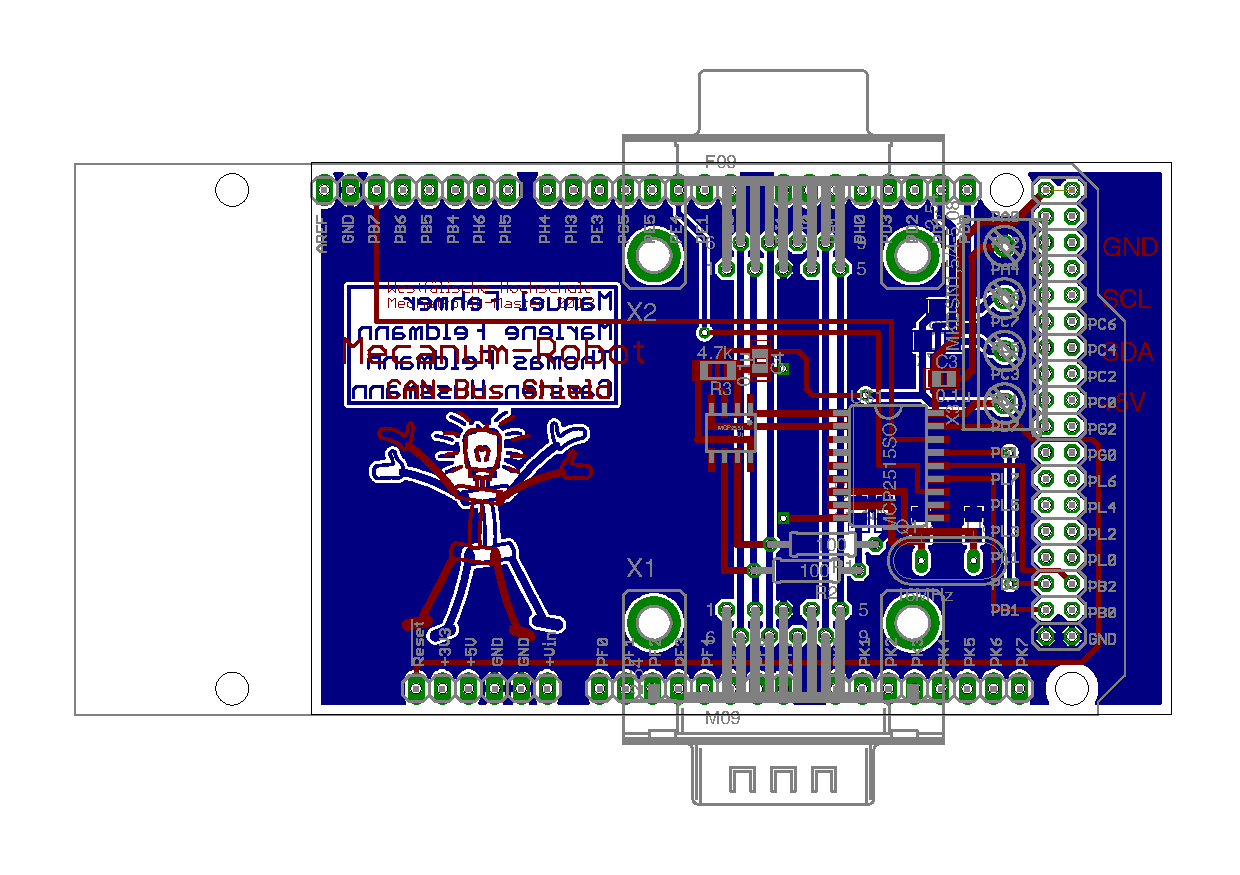
\includegraphics[width=0.8\textwidth]{Abbildungen/CAN-Shield-Layout}
\caption[CAN-Shield-Layout]{CAN-Shield-Layout}
\label{fig:CAN-Shield-Layout}
\end{figure}

\begin{figure}[H]
\centering
 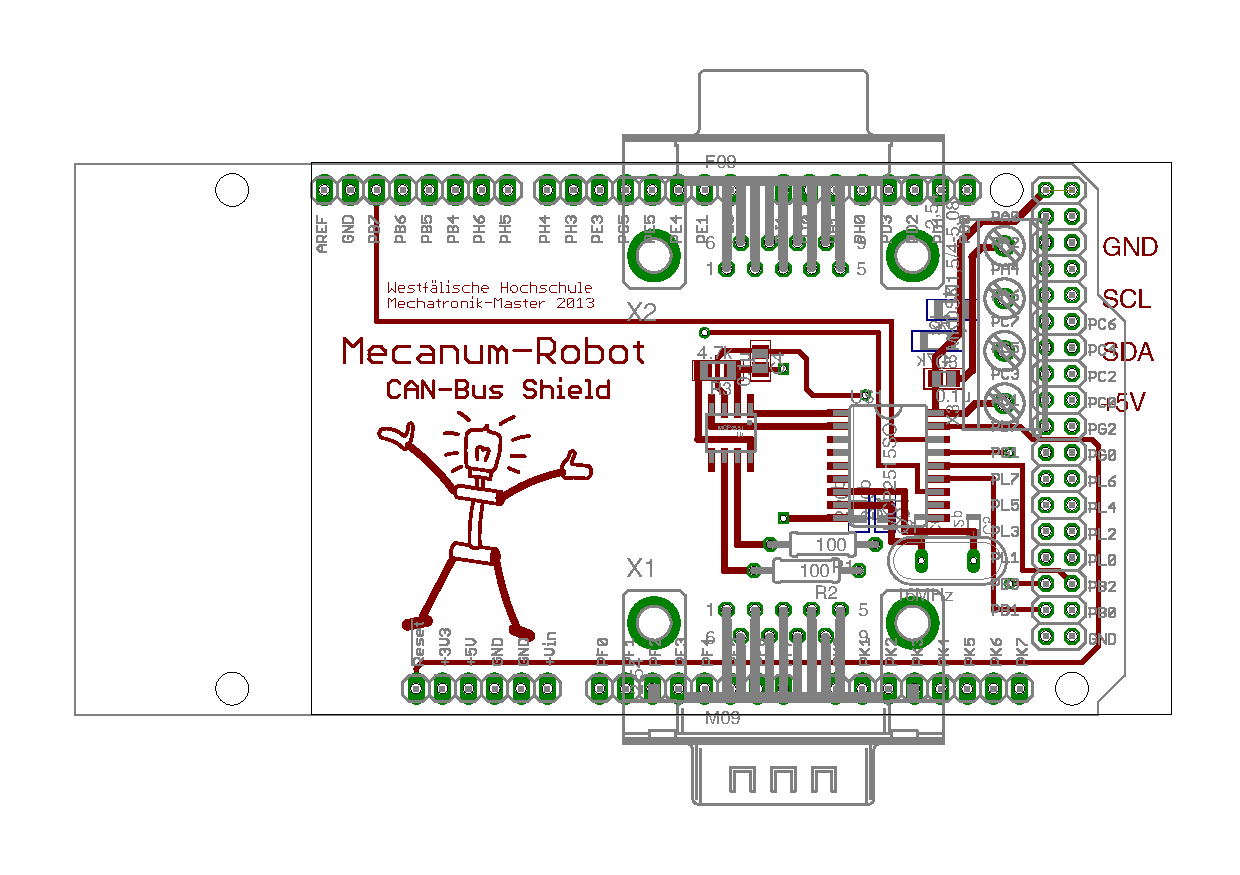
\includegraphics[width=0.8\textwidth]{Abbildungen/CAN-Shield-Layout-Top}
\caption[CAN-Shield-Top-Layer]{CAN-Shield-Top-Layer}
\label{fig:CAN-Shield-Layout-Top}
\end{figure}

\begin{figure}[H]
\centering
 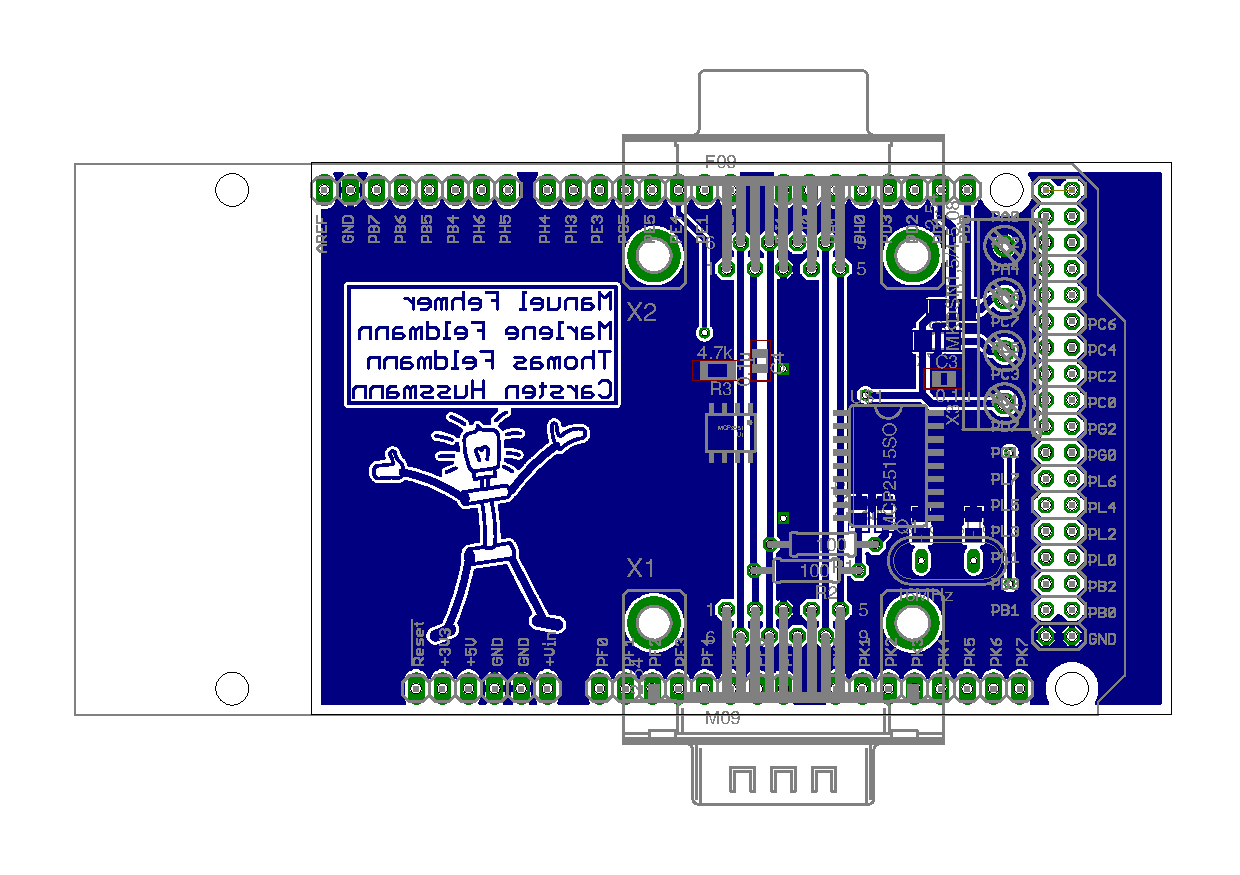
\includegraphics[width=0.8\textwidth]{Abbildungen/CAN-Shield-Layout-Bottom}
\caption[CAN-Shield-Bottom-Layer]{CAN-Shield-Bottom-Layer}
\label{fig:CAN-Shield-Layout-Bottom}
\end{figure}

\subsection{Drahtlose Navigation auf dem Betriebsgelände}
\label{sec:Navigation}
\begin{figure}
\centering
    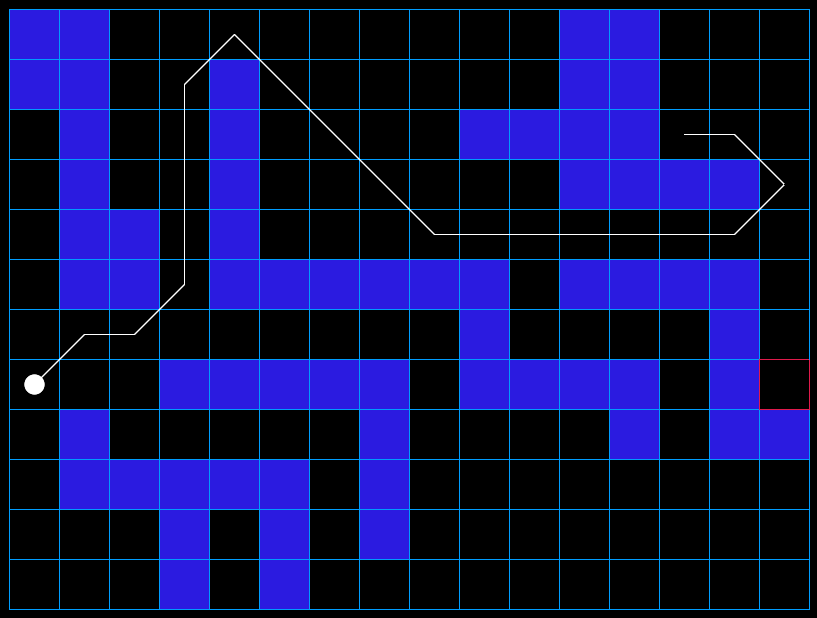
\includegraphics[width=.8\textwidth]{Abbildungen/Dijkstra}
    \caption[Dijkstra]{Pathfinding-Algorithmus nach Dijkstra}
    \label{fig:Dijkstra}
\end{figure}
Um die Navigation auf dem Betriebsgelände zu ermöglichen, muss der Roboter stets seine Position und Ausrichtung im Raum kennen. Dazu kann eine Deckenkamera und eine entsprechende Markierung auf dem Roboter eingesetzt werden.

In Abbildung~\ref{fig:Dijkstra} ist ein Ergebnis des Dijkstra Pathfinding Algorithmus\footnote{http://www.smellycatcards.com/index.php/welcome/pathfinding} dargestellt.
Das Betriebsgelände wird hier in befahrbare (schwarz) und nicht befahrbare Bereiche (blau) eingeteilt. Die resultierende Fahrtvorgabe (weiße Linie) ist die kürzeste Verbindung zwischen Start- und Zielpunkt in der Halle (Ob nur senkrechte oder auch diagonale Fahrten zugelassen werden, kann in der der Implementierung des Algorithmus angepasst werden).

Die nicht befahrbaren Bereiche können auf diese Weise dynamisch angepasst werden. So können auch die Deckenkamera und die auf dem Roboter integrierten Sensoren zur Hindernisserkennung hinzugezogen werden.

Der Roboter soll sich im Akkubetrieb kabellos bewegen können. Für die Kommunikation ist daher die Einrichtung eines Funknetzwerks nötig. Dies kann durch ein auf den Arduino aufgestecktes Ethernet-Shield realisiert werden, wegen der begrenzten Rechenleistung und Speicherkapazität des Arduinos wird diese Möglichkeit aber unnötig kompliziert.
Einfacher wäre die Integration eines Kleinrechners auf Basis von Embedded Linux\footnote{Beispielsweise dem Raspberry Pi: http://www.raspberrypi.org}. Die Server-Framework \emph{Flask\footnote{http://flask.pocoo.org}} auf Basis der Programmiersprache \emph{Python\footnote{http://www.python.org}} stellt eine einfache Möglichkeit dar, den Roboter über ein Webinterface zugänglich zu machen. Über die Library \emph{PySerial\footnote{http://pyserial.sourceforge.net}} kann die in Kapitel~\ref{sec:API} erläuterte API genutzt werden, am Arduino und dem CAN-Bus Shield wären somit keine Änderung notwendig.



\end{document}
